\documentclass[a4paper,14pt]{extarticle}
\usepackage{../../tex-shared/report-layout}

\renewcommand{\mylabnumber}{2}
\renewcommand{\mylabtitle}{Исследование архитектуры универсального 8-разрядного 
микропроцессора}
\renewcommand{\mysubject}{Технические средства информационных систем}
\renewcommand{\mylecturer}{Дрозин А.Ю.}

\begin{document}
\begin{titlepage}
    
    \thispagestyle{empty}
    
    \begin{center}
        
        Министерство науки и Высшего образования Российской Федерации \\
        Севастопольский государственный университет \\
        Кафедра ИС
        
        \vfill

        Отчет \\
        по лабораторной работе №\mylabnumber \\
        \enquote{\mylabtitle} \\
        по дисциплине \\
        \enquote{\MakeTextUppercase{\mysubject}}

    \end{center}

    \vspace{1cm}

    \noindent\hspace{7.5cm} Выполнил студент группы ИС/б-17-2-о \\
    \null\hspace{7.5cm} Горбенко К. Н. \\
    \null\hspace{7.5cm} Проверил \\
    \null\hspace{7.5cm} \mylecturer

    \vfill

    \begin{center}
        Севастополь \\
        \the\year{}
    \end{center}

\end{titlepage}
\section{Цель работы}
Исследовать архитектуру и основные блоки 8-разрядного процессора.
Исследовать взаимодействие основных блоков процессора при выполнении команд
разных типов. Приобрести навыки написания и отладки ассемблерных программ в
эмуляторе KP580 Emulator.

\section{Задание на работу}
\begin{enumerate}
    \item Изучить архитектуру МП КР580ВМ80.
    \item Изучить основные команды МП КР580ВМ80.
    \item Задавая различные команды (запись в регистр и в пару регистров,
    пересылки данных, суммирования при наличии переноса, чтения и записи в память,
    записи в стек, обращения к памяти путем косвенной адресации и др.) исследовать
    наличие и вид сигналов и данных на шинах процессора, содержимое регистров,
    значение флагов и взаимодействие блоков МП КР580ВМ80 в ходе выполнения команд.
\end{enumerate}

\section{Ход работы}
Процессор состоит из АЛУ, аккумулятора A, регистров общего назначения B, C, D, E, H, L.
Эти компоненты соединены шинами (данных, адреса, управления) мужду собой и с ОЗУ.
На рисунке \ref{fig:scheme} изображена структурная схема процессора МП КР580ВМ80.

\begin{figure}[H]
    \centering
    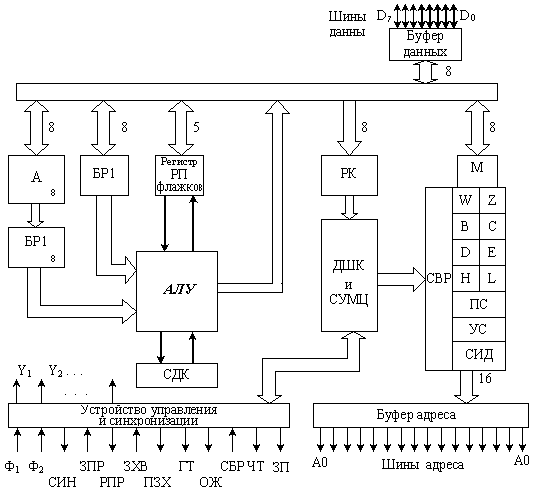
\includegraphics[width=.8\linewidth]{scheme}
    \caption{Структурная схема микропроцессора МП КР580ВМ80}
    \label{fig:scheme}
\end{figure}

\subsection{Изучение команд процессора}
\subsubsection{Команды пересылки данных}
Выполним команды пересылки данных. Команда MOV выполняет пересылку байта данных от
источника к приемнику. Команда MVI выполняет запись в источник из регистра данных.
\begin{figure}[H]
    \centering
    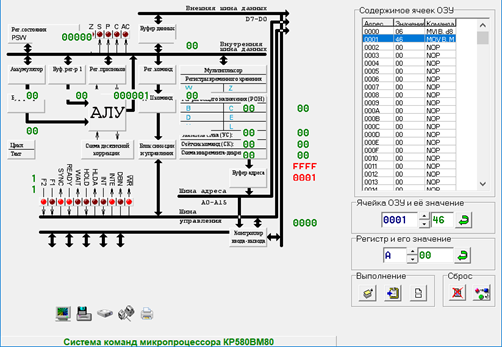
\includegraphics[width=.8\linewidth]{mov}
    \caption{Выполнение команд пересылки данных}
    \label{fig:mov}
\end{figure}

\subsubsection{Команда LXI}
Команда LXI загружает второй и третий байты команды в регистровую пару.
Производится запись числа 0007 в регистры DE.
\begin{figure}[H]
    \centering
    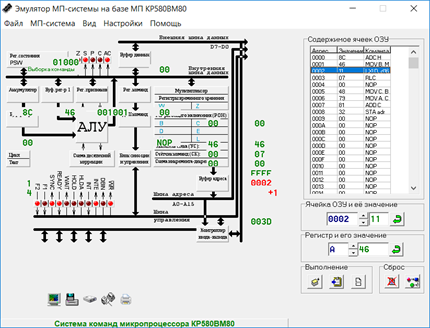
\includegraphics[width=.8\linewidth]{lxi}
    \caption{Выполнение команды LXI (Адрес 0002)}
    \label{fig:lxi}
\end{figure}

\subsubsection{Команда ADD}
Следующая команда ADD производит сложение содержимого аккумулятора с
содержимым регистра С: (A) $\leftarrow$ (A) + (С). В аккумуляторе лежало число
46\textsubscript{16} , к нему прибавляем значение регистра, тоже 46\textsubscript{16}.
В результате в аккумуляторе будет лежать число 8С\textsubscript{16}.
Так как перенос в старший разряд не произведен, то индикатор
признака переноса С не светится.
\begin{figure}[H]
    \centering
    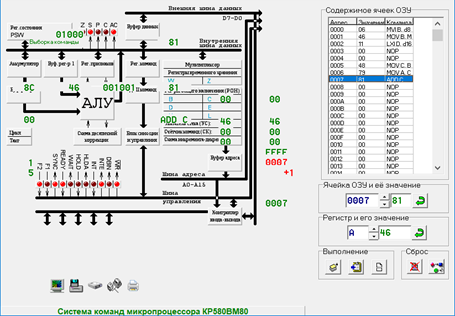
\includegraphics[width=.8\linewidth]{add}
    \caption{Выполнение команды ADD (Адрес 0007)}
    \label{fig:add}
\end{figure}

\subsubsection{Команда LDAX}
Команда LDAX пересылка из ячейки памяти, адрес которой записан в регистровой
паре DE, в аккумулятор. В регистрах лежит адрес «0007», а по этому адресу лежит
значение «81», которое и запишется в аккумулятор.
\begin{figure}[H]
    \centering
    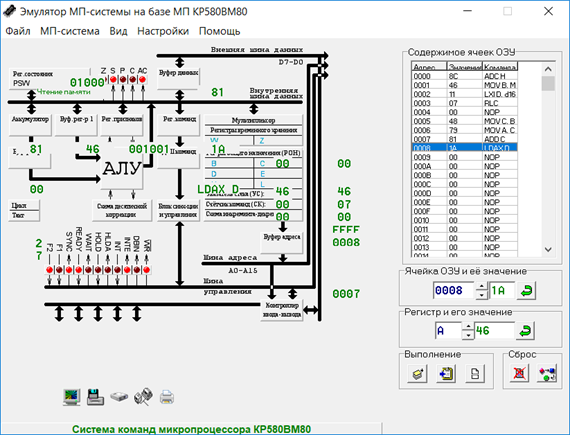
\includegraphics[width=.8\linewidth]{ldax}
    \caption{Выполнение команды LDAX (Адрес 0008)}
    \label{fig:ldax}
\end{figure}

\subsubsection{Команда STA}
STA выполняет пересылку из аккумулятора в ячейку памяти, адрес которой указан
во втором и третьем байтах команды. В нашем случае процессор должен записать
значение «81» в ячейку памяти с адресом «0000».
\begin{figure}[H]
    \centering
    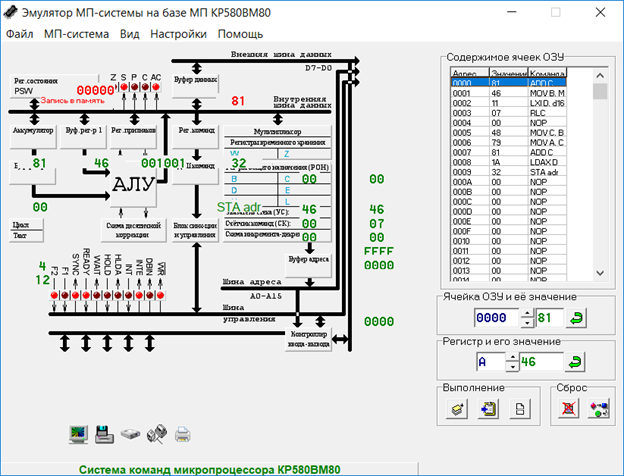
\includegraphics[width=.8\linewidth]{sta}
    \caption{Выполнение команды STA (Адрес 0009)}
    \label{fig:sta}
\end{figure}

\section*{Выводы}
В ходе выполнения лабораторной работы была исследована архитектура 8-разрядного
процессора. Исследовано взаимодействие основных блоков процессора при выполнении
команд разных типов. Были приобретены практические навыки написания и отладки
ассемблерных программ в эмуляторе KP580 Emulator.

\end{document}